\section{Sistemi Peer-to-Peer}
\subsection{Introduzione}
Il paradigma P2P, abilita due o più entità a collaborare spontaneamente in un network di peers("nodi uguali"), usando informazioni e metodi di comunicazioni appropriati senza l'utilizzo di una autorità centralizzata!!

Si può fare distinzione fra tipi di reti P2P:
\begin{itemize}
    \item sistemi p2p dove gli utenti controllano le proprie risorse
    \item p2p dove i dati sono controllati da server centralizzati
    \item p2p ibridi con parte di utenza decentralizzata e parte server
\end{itemize}

Le attività dei sistemi p2p sono guidate dal'ambiente(environment) e dai feedback interni alla rete.
\begin{figure}[h!]
    \centering
    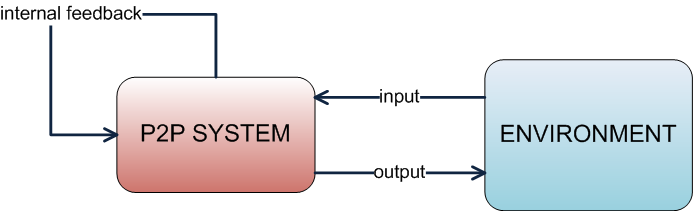
\includegraphics[width=0.5\linewidth]{imgs/5 - p2p.png}
    \label{fig:p2p}
    \caption{Struttura p2p}
\end{figure}
Gli input dell'environment targhettano pochi peer della rete.
I nodi p2p quando ricevono dei dati dalla rete possono essere progrmmati in due modi:
\begin{itemize}
    \item statico: una volta settato il nodo svolgere le sue funzioni sempre nello stesso nodo
    \item Piano adattivo: poù cambaire in corso d'opera in base a cosa gli viene detto dall'environment
\end{itemize}

\subsubsection{Variabili di stato}
Un sistema p2p è una rete di peers, quando si entra nella rete, ogni peer si connette con tutti gli altri.
I peer condividono risorse come: banda, cpu, storage, ecc.

\begin{itemize}
    \item Risorse replicabili: dati
    \item risorse consuabili: storage, cpu ecc
    \item Servizi distribuiti: servizi che rihiedono l'esecuzione su molti peer
    \item servizi locali: funzioni esposte da un peer per permettere l'accesso alle risorse locali
\end{itemize}

Ogni peer ha un tempo di vita $L$ che viene modellata secondo: il rolo del peer, disponibilità della risorsa eed eventi non predicibili.
Variabili misurate dal peer:
\begin{itemize}
    \item uso delle risorse condivise
    \item tempo di risposta dei vicini
    \item query hit ratio (QHR)
\end{itemize}

Variabili impostate dal pper:
\begin{itemize}
    \item dimensione della tabella di instradamento
    \item strategia di riempimenti delle tabelle di instradamento
    \item algoritmo per l'instradamento dei messaggi
    \item banda di unload
    \item banda download
\end{itemize}

Si usano metodi stocastici per misurare la distribuzione delle risorse e la loro popolarità.
\subsubsection{problemi di design}
La topologia della rete, il grado di centralizzazione e l'instradamento del messaggio sono cruciali per le operazioni del sistema(scalabilità, sicurezza, tolleranza agli errori, auto maantenimento).

Efficacia ed efficenza:
\begin{itemize}
    \item scalability
    \item boostrapping
    \item connectivity management
    \item search performance
    \item consitency
    \item stability
    \item load balance
    \item asymmetric bandwidth
\end{itemize}

Sicurezza:
\begin{itemize}
    \item Attacchi passivi
        \begin{itemize}
            \item eavrsdropping
            \item traffic analysis
        \end{itemize}
    \item Attacchi attvi
    \begin{itemize}
        \item spoofing
        \item man in the middle
        \item playback or replay
        \item local data alteration
        \item no forwarding
        \item free riding
        \item distributed denial of service (DDOS)
        \item network poisoning
    \end{itemize}
    \item sicurezza
    \begin{itemize}
        \item trust managment
    \end{itemize}
\end{itemize}

\subsubsection{Strategia di design per gli schemi di overlay}
nei sistemi p2p la posizione dell'informazione gioca un ruolo importante per l'overlay scheme.
\begin{itemize}
    \item server centrale
    \item peer to peer
    \item salvato in locale e non pubblico
\end{itemize}
Gli schemi di overlay:
\begin{itemize}
    \item modello ibrido(HM)
    \item modello decentralizzato non strutturato(DUM)
    \item modello decentralizzato strutturato(DSM)
\end{itemize}

\begin{figure}[h!]
    \centering
    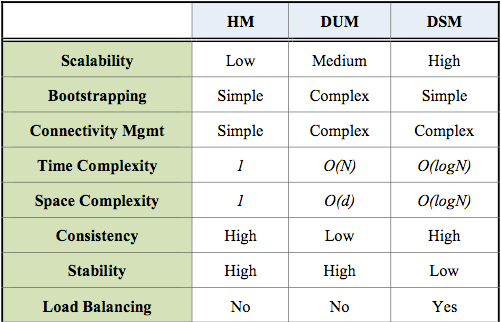
\includegraphics[width=0.8\linewidth]{imgs/6 - strategie di design p2p.png}
    \label{fig:designStrategiesP2p}
    \caption{Strategie di design reti p2p}
\end{figure}

\begin{figure}[h!]
    \centering
    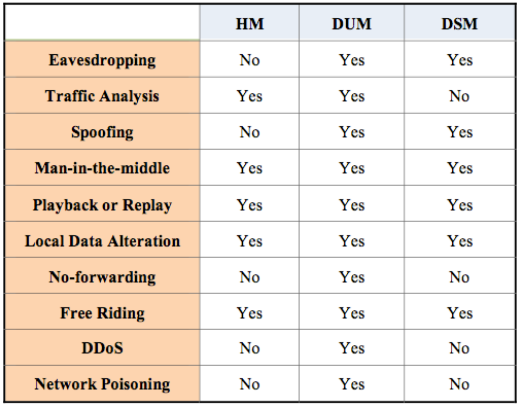
\includegraphics[width=0.8\linewidth]{imgs/7 - overlay design.png}
    \label{fig:designOverlayP2p}
    \caption{Strategie di design per gli schemi di overlay}
\end{figure}

\subsubsection{Modello ibrido(HM)}
I peer sono connessi a uno o più nodi centralizzati(server) che pubblicano le risorse.
Se un peer ha bisogno di un dato in un server, manda la richiesta, gli ritorna una risposta con il percorso da prendere e prende il dato.
Se il serve non è unico, le richieste potrebbere essere instradate a server vicini.
Esempi: eMule, BitTorret ecc
\begin{figure}[h!]
    \centering
    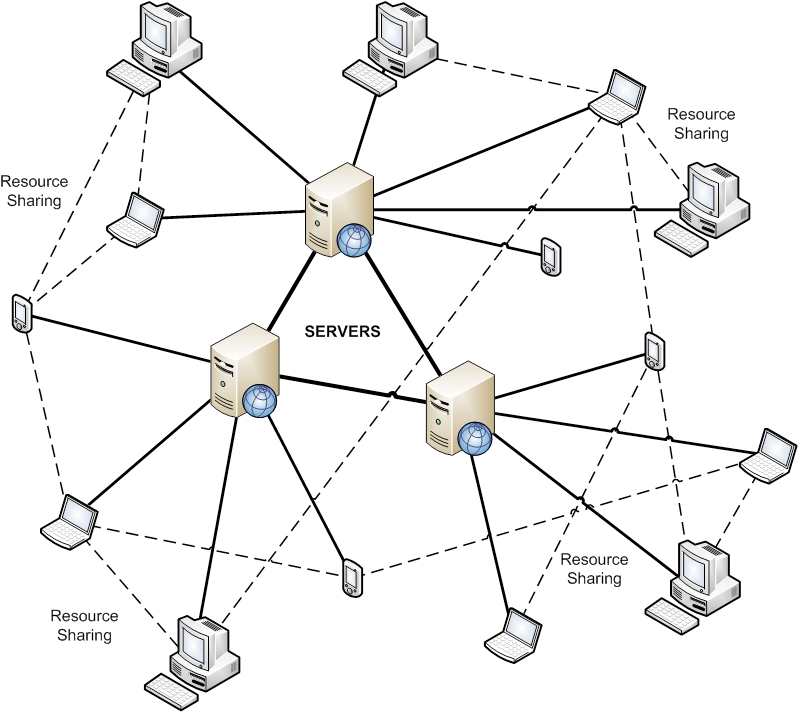
\includegraphics[width=0.5\linewidth]{imgs/8 - HM.png}
    \label{fig:p2pHM}
    \caption{Modello ibrido}
\end{figure}
\subsubsection{Modello decentralizzato non strutturato(DUM)}
Ogni peer propaga la richiesta ai peer adiacenti(simile alla strategia flooding) efficace in comunità piccole ma non scalabile.
Per migliorare la scalabilità si fa cache delle risorse recenti.
Se un'identità viene aggiunta al dato i peer possono non propagare il dato.
In network grandi è necessario un time-to-live(TTL) per evitare che un pachetto stalli per sempre.
\subsubsection{Modello decentralizzata non strutturato(DUM)}
\begin{figure}[h!]
    \centering
    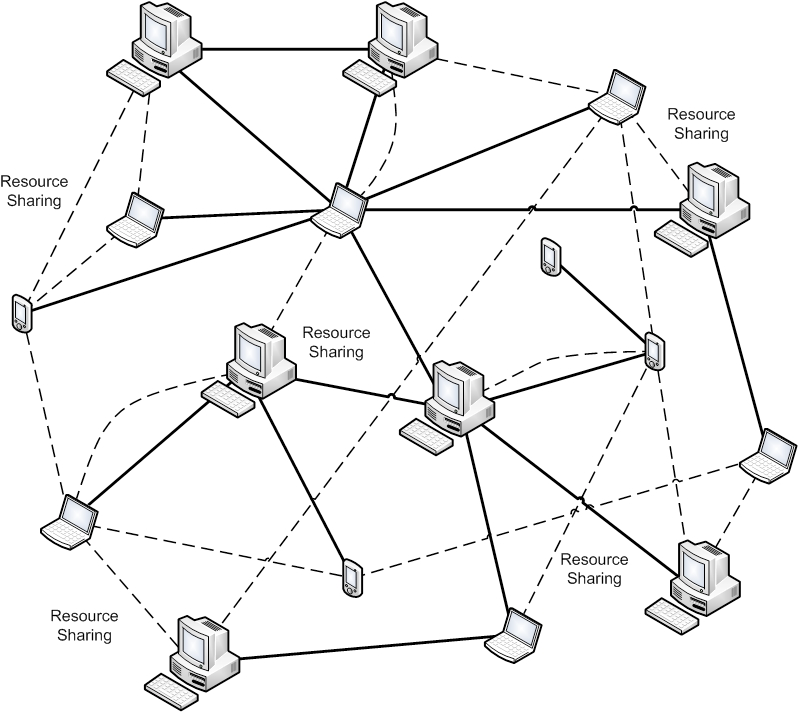
\includegraphics[width=0.5\linewidth]{imgs/9 - DUM.png}
    \label{fig:p2pDUM}
    \caption{Modello Decentralizzato non strutturato}
\end{figure}
\subsubsection{Modello decentralizzato strutturato(DSM)}

Un protocollo globale fa si che ogni noda possa raggiungere la risorsa efficacemente,
La tecnica più comune è una hash table distribuita dove ogni risorsa è identificata da una chiave univoca associata ad una chiave di decriptazione.

Ogni peer ha un ID assegnato ed è responsabile di tenere l'id salvato.

\textbf{Pubblicazione}: la descrizione di ua risorsa e la sua coppia chiave risorsa vengono messe nelle tabelle di routing adiacenti all'id del peer. 
Questo processo viene ripetuto finche ogni peer adiacente conosce l'id del peer in questione.


Il DSM è molto più decentralizzato del DUM.

\textbf{Lookup}: la query viene propagata attraverso i peer con l'ID della risorsa.

Pratica comune per stabili la lunghezza dei percorsi fra nodi è:

\begin{center}
    \begin{tabular}{| c | c |}
        \hline
        Nodi & Route Lenght \\
        \hline
        $O(1)$ & $O(N)$ \\
        \hline
        $O(\log(N))$ & $O(\frac{\log(N)}{\log(\log(N))})$ \\
        \hline
        $O(\log(N))$ & $O\log(N)$ \\
        \hline
        $O\sqrt(N)$ & $O(1)$ \\
        \hline
    \end{tabular}
\end{center}

\begin{figure}[h!]
    \centering
    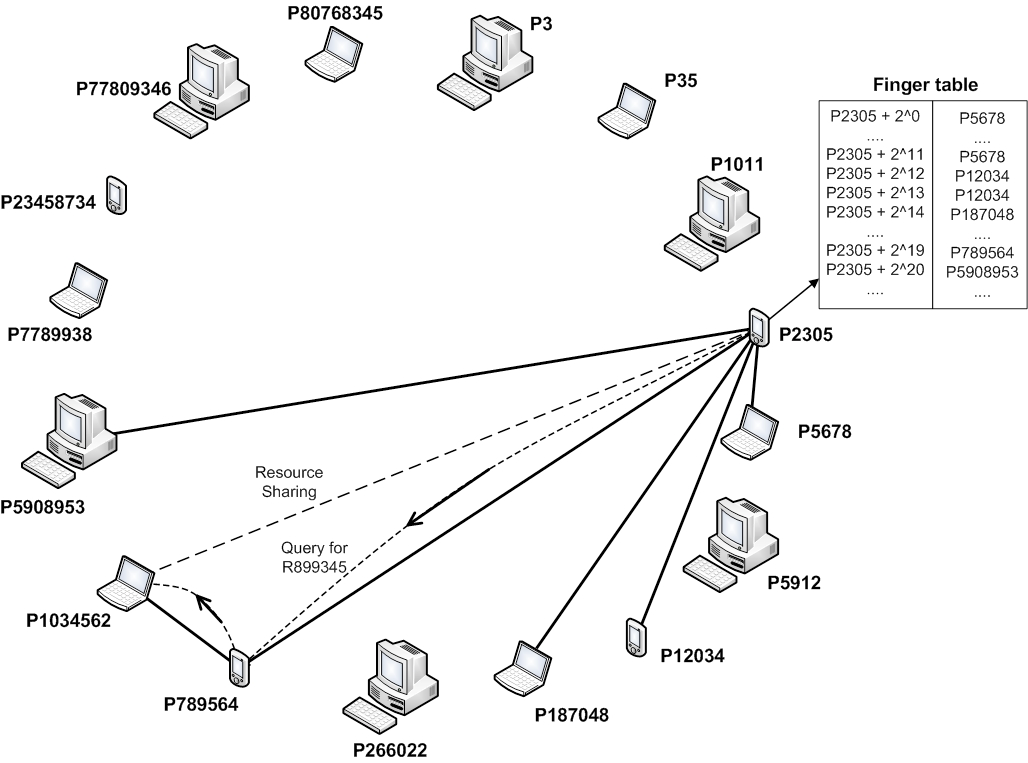
\includegraphics[width=0.5\linewidth]{imgs/10 - DSM.png}
    \label{fig:p2pDSM}
    \caption{Modello Decentralizzato strutturato}
\end{figure}

\subsubsection{Schema overaly stratificato}
In una Struttura di peers con multi layer, si utilizzano dei protocolli per permettere la comunicazione fra vari layer.

\begin{figure}[h!]
    \centering
    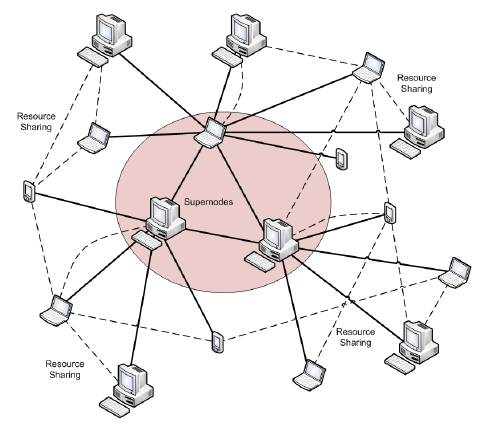
\includegraphics[width=0.5\linewidth]{imgs/11 - layer overlay scheme.png}
    \label{fig:overlay}
    \caption{Schema di overlay a strati}
\end{figure}

